\documentclass{article}

\usepackage[dblblindworkshop,nonanonymous]{neurips_2026}
\workshoptitle{Interpretability for Discovery}

\usepackage[utf8]{inputenc}
\usepackage[T1]{fontenc}
\usepackage{hyperref}
\usepackage{url}
\usepackage{booktabs}
\usepackage{amsfonts}
\usepackage{amsmath}
\usepackage{nicefrac}
\usepackage{microtype}
\usepackage{xcolor}
\usepackage{graphicx}

\title{Causal Steering of Protein Language Models: \\
When Correlational Validation Fails, and How to Catch It}

\author{%
  Dmitriy Ivkov \\
  University of Michigan \\
  \texttt{divkov@umich.edu}
}

\begin{document}

\maketitle

\begin{abstract}
Activation steering has recently been shown to reproduce a known protein
property (thermostability) in ESM2-650M via difference-of-means vectors.
We ask whether a scoring proxy's correlation with real experimental
labels predicts whether steering toward it actually works, and find the
answer is no. Under a pre-registered six-criterion protocol testing five
novel target properties, our best-validated proxy (binding affinity,
$r=0.80$ held-out) steers nothing, while a substantially weaker one
($r=0.22$, catalytic activity) produces a robust, three-seed-replicated
effect. This mirrors an independent, component-level finding in the same
model family: attention heads ranked by correlation with real 3D
contacts show near-zero relationship to their causal ablation effect. We
show that a single-seed steering result can mislead in
criterion-specific ways. For one target, the effect direction replicates
across three seeds, but the residue-exclusion check passes on only two.
We also introduce a lightweight diagnostic based on steering-vector
cosine similarity across targets. It explains an otherwise unexplained
ambiguous result as a geometric echo of a different property's validated
direction. We release the full protocol, all target harnesses, and the
seed-replication data.
\end{abstract}

\section{Introduction}

Difference-of-means activation steering adds a direction to a model's
residual stream. The direction is built from the mean activation
difference between high- and low-property example groups. This method
reproduces known thermostability biology in ESM2-650M
\citep{huang2025steering}. We ask the natural follow-up: does a scoring
proxy's correlation with real labels predict whether steering toward a
new property works? Across five novel targets under one
pre-registered protocol, the best-validated proxy in our study ($r=0.80$,
binding affinity) produces a flat null effect, while a substantially
weaker proxy ($r=0.22$, catalytic activity) produces a clean,
three-seed-replicated effect. This mirrors an independent,
component-level result: Vig et al.\ \citep{vig2021bertology} found an
attention head whose correlation with real 3D contacts is 12.9$\times$
enrichment, explicitly flagged as untested causally; ablating it gives an
effect indistinguishable from a low-correlation control, and a full
480-head sweep ranks the correlational top pick 313th of 480 by actual
causal effect. Two levels, two techniques, one lesson: correlational
signal is evidence about representations, not about intervention. Our
contribution is the audit discipline needed to trust a causal claim
here, demonstrated via two near-misses caught in our own pipeline before
they could be reported as clean results.

\section{Method}
\label{sec:method}

We lock six criteria before testing any target and compute them
automatically. Criterion 1 requires the real direction to beat a
matched-norm random control via paired bootstrap with 10{,}000 resamples.
Criterion 2 requires a monotonic dose-response across at least three
strengths within a safe range (\S\ref{sec:cases}). Criterion 3 requires
the effect to survive residue-exclusion, and criterion 4 requires the
proxy to be validated against real labels before the run. Criterion 5
requires the result to beat the best existing technique when one exists,
and criterion 6 requires at least 150 held-out sequences. A target failing
any criterion is a KILL; one passing 1--2 but failing 3 or 4 is AMBIGUOUS.

\section{The Central Finding: Proxy Validity Does Not Predict Causal Effect}
\label{sec:sweep}

\begin{table}[t]
\centering
\caption{Five novel targets. Proxy $r$: Pearson correlation vs.\ real
labels, held-out, before any steering run.}
\label{tab:sweep}
\small
\begin{tabular}{@{}p{2.3cm}p{1.0cm}p{2.6cm}p{1.9cm}@{}}
\toprule
Target & Proxy $r$ & Steering result & Verdict \\
\midrule
Binding affinity & 0.80 & flat null, all $\alpha$ & KILL \\
Catalytic activity & 0.22 & PASS, 3/3 seeds & PASS \\
Intrinsic disorder & 0.45 & 3/3 direction; 2/3 robustness & PASS* \\
Immunogenicity & $\leq$0.10 & not run & KILL (pre-run) \\
Expression yield & 0.31 & fails residue-exclusion & AMBIGUOUS \\
\bottomrule
\end{tabular}

\smallskip
\footnotesize *PASS on criteria 1,2,4,6, and 2/3 seeds on criterion 3.
\end{table}

\begin{figure}[t]
\centering

\includegraphics[width=0.62\linewidth]{figures/fig2_proxy_vs_effect.pdf}
\caption{Proxy validity vs. steering effect size (Cohen's $d$,
$\alpha=0.5$). The best-validated proxy (binding affinity, $r=0.80$)
gives the smallest effect; a proxy less than half as strong (catalytic
activity, $r=0.22$) gives one of the two largest. No positive trend.}
\label{fig:proxy-vs-effect}
\end{figure}

\paragraph{Binding affinity.} We use ProteinGym DMS data for KRAS binding
to a DARPin. Its mutational-sensitivity-weighted proxy is validated more
rigorously than any other target here: $r=0.80$ held-out, a
weight-shuffle null of $r=-0.001$, held-out-position generalization of
$r=0.54$, and single-to-double-mutant extrapolation of $r=0.70$. Yet the
steering effect is a flat null at every $\alpha$, with zero degenerate
sequences at any strength. A plausible mechanism is that the
vector-building groups are single-backbone point mutants, only 1--2
residues from a shared reference. Difference-of-means therefore has
little compositional signal to use. The mean compositional distance
between low and high groups is $0.003$, compared with $0.02$--$0.05$ for
the three cross-protein targets below.

\paragraph{Catalytic activity.} On the cross-protein DLKcat dataset, a
glycine-minus-arginine proxy matches the published activity-stability
tradeoff in enzymology. It is the weakest proxy among the four runnable
targets, with $r=0.22$, but produces a clean, monotonic,
residue-robust effect
(Figure~\ref{fig:dose-response}, left) replicated identically across
three independent seeds. It is the only target with fully unanimous
seed robustness.

\paragraph{Intrinsic disorder.} The DisProt proxy uses the TOP-IDP scale.
It is the strongest proxy here, with $r=0.45$ and a per-residue AUC of
$0.71$. The effect is significant and monotonic on all 3 seeds
(Figure~\ref{fig:dose-response}, right), but its residue-exclusion check
passes on only 2. Those seeds retain 36--42\% of the magnitude. On the
third seed, 10\% is retained and the confidence interval crosses zero.
Existence and direction are seed-stable, but the artifact check is not.

\begin{figure}[t]
\centering
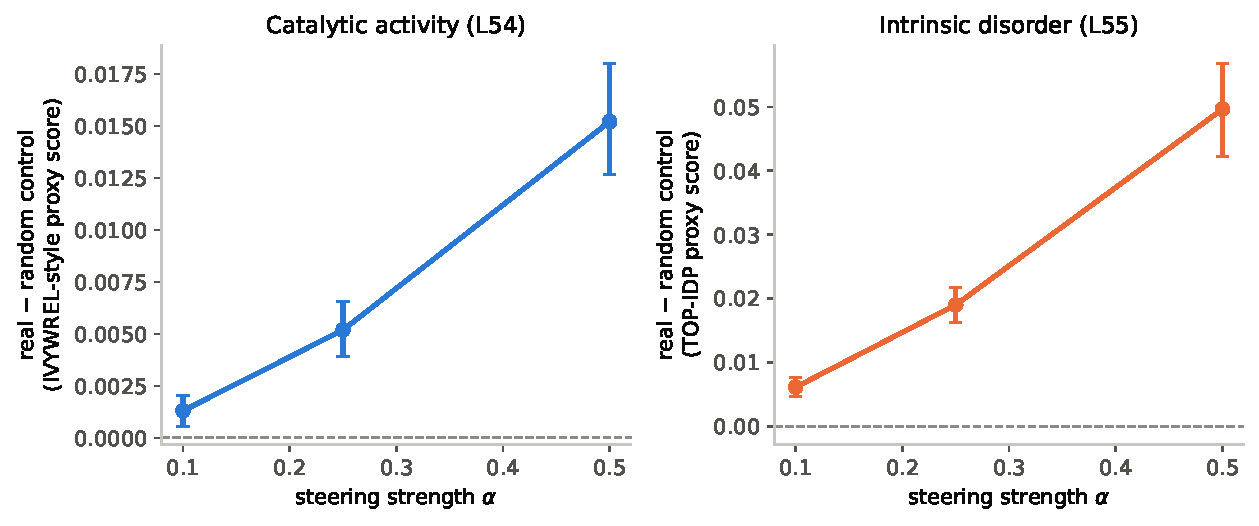
\includegraphics[width=\linewidth]{figures/fig1_dose_response.pdf}
\caption{Dose-response, the two targets passing criterion 2. Both
monotonic, 95\% bootstrap CIs bounded away from zero throughout.}
\label{fig:dose-response}
\end{figure}

\paragraph{Immunogenicity.} Across four IEDB tiers, proxies predictive on
a surrogate binding-affinity tier ($r=0.37$--$0.43$) collapse to near
chance on the real T-cell-response endpoint ($r\leq0.10$). A
full-length-antigen proxy reaches $r=0.38$, but organism identity explains
58\% of the apparent signal. Its correlation flips to $r=-0.32$ once
organism is held out of cross-validation. The target is killed before any
steering run.

\paragraph{Expression yield.} The eSol net-charge-deviation proxy
validates at $r=0.31$--$0.34$. Its effect is significant and
dose-responsive but collapses under residue-exclusion. Rather than
discarding this result, we compute steering-vector cosine similarity
against every other target: $+0.38$ overall with intrinsic disorder's
vector, rising to $+0.56$--$0.67$ at the three deepest layers. This is
consistent with literature showing that disordered regions reduce
solubility and expression. The result is best read as a partial echo of disorder's
already-validated effect through a more collapse-prone proxy, not a
sixth steerable property.

\section{Self-Correction Case Studies}
\label{sec:cases}

\paragraph{A spurious pass from an unsafe comparison.} Testing whether
restricting steering to the 5 layers previously found causally necessary
preserves the full 33-layer effect, a first pass selected its
best-performing $\alpha$ from the whole tested range, including
$\alpha\geq1.0$, and reported a clean pass at $\alpha=2.0$. This was
comparison artifact. At that $\alpha$, the 33-layer arm had already fully
collapsed into degenerate output, leaving zero non-degenerate sequences.
The 5-layer arm had not collapsed, so it won only by breaking down later.
After restricting the comparison to a range where neither arm has
collapsed and rerunning end to end, the 5-layer subset retains only
43--59\% of the full effect.

\paragraph{A criterion passing on only 2 of 3 seeds.} The disorder target's
residue-exclusion check (\S\ref{sec:sweep}) is seed-sensitive even though
the headline effect is not. A single seed could have reported either a
false unanimous pass or a false kill on this criterion. Only a multi-seed
rerun reveals the instability.

\section{Related Work}

\citet{huang2025steering} validate this steering method on
thermostability; we extend it to five new properties under a
pre-registered protocol and test, to our knowledge for the first time,
whether proxy correlation strength predicts steering success across
unrelated properties. \citet{vig2021bertology} identify the head we redo
as a genuine causal test. \citet{adams2025mechanistic} train SAEs on
ESM-2 and show through correlational linear probing that thermostability
and localization determinants are identifiable in SAE feature space.
Their one steering check is a coherence test, not validation against a
real label, and their discussion states ``investigating how to steer the
model in useful ways remains an open direction for future work.'' We
answer a version of that for a non-SAE mechanism, specifically for
whether correlational validity predicts causal usefulness.

\section{Discussion}

Every steering result here is causal about the model's activation space.
It reflects a real intervention evaluated against a random-direction
control and a residue-exclusion check, but it is not validated against a
wet-lab assay. A PASS means ``causally steers a validated proxy,'' not
``causally engineers the biological property.'' The vector-geometry
check that explained the expression-yield result requires only one extra
embedding pass. It is worth running by default whenever multiple targets
are tested together.

All experiments use one model, ESM2-650M, at one scale, and all proxies
are compositional heuristics. Each target's proxy was selected as the best
of several candidates on the same held-out split used for its reported
$r$, so the values should be read as upper bounds. We ran many
significance tests without a multiple-comparisons correction, although
requiring multi-alpha and multi-seed agreement for a PASS partly
mitigates this issue. Seed robustness was checked for only two of five
targets, and generated sequences received no structural or functional
plausibility check.

\section{Conclusion}

Correlational validity does not predict causal effect when tested at two
levels of the same model class. This applies both to an attention head's
biological alignment and to a proxy's correlation with real labels. Proxy
validation strength is not a reliable filter for which targets are worth
attempting, and a single steering run should not be trusted without a
seed-robustness check where the result matters downstream.

\section*{Responsible-use statement}
This work identifies methodological pitfalls in causally validating
activation-steering claims on protein language models and does not
introduce a new capability for generating harmful biological sequences;
all target properties studied (thermostability, binding, catalysis,
disorder, immunogenicity, expression) are common protein-engineering
objectives with dual-use risk no greater than the underlying published
steering method \citep{huang2025steering} we extend. We see no additional
mitigation specific to this paper's contribution beyond standard
biosecurity practice already governing protein-language-model research.

\bibliographystyle{plainnat}
\bibliography{reference}

\end{document}
